\documentclass[utf8,english]{gradu3}
% If you are writing a Bachelor's Thesis, use the following instead:
%\documentclass[utf8,bachelor,english]{gradu3}

\usepackage{graphicx} % for including pictures

\usepackage{amsmath} % useful for math (optional)

\usepackage{booktabs} % good for beautiful tables

% NOTE: This must be the last \usepackage in the whole document!
\usepackage[bookmarksopen,bookmarksnumbered,linktocpage]{hyperref}

\addbibresource{bibliography.bib} % The file name of your bibliography database

\begin{document}

\title{Machine learning based automatic analysis of physics instruction quality}
\translatedtitle{Koneoppimispohjainen automaattinen fysiikan opetuksen laadun analyysi}
\studyline{Educational Technology}
\avainsanat{%
  TODO: Avainsanat}
\keywords{TODO: Keywords}
\tiivistelma{%
  TODO: Tiivistelmä
}
\abstract{%
  TODO: Abstract
}

\author{Aleksander Lempinen}
\contactinformation{\texttt{aleksander.lempinen@outlook.com}}
% use a separate \author command for each author, if there is more than one
\supervisor{Tommi Kärkkäinen}
\supervisor{Daniela Caballero}
\supervisor{Jouni Viiri}


% use a separate \supervisor command for each supervisor, if there
% is more than one

\maketitle

\begin{thetermlist}
\item[TODO] TODO: Glossary
\item[ASR] Automatic Speech Recognition
\item[HMM] Hidden Markov Model
\item[LSTM] Long Short-Term Memory 
\item[ML] Machine Learning
\item[NLP] Natural Language Processing
\item[RNN] Recurrent Neural Network
\item[NLTK] Natural Language Toolkit
\end{thetermlist}

\mainmatter


%--------------------------------------------------------------------------------


\chapter{Introduction}
Automating the laborious and subjective process of analysing classroom speech data has potential for improving physics instruction quality and providing new tools for physics teacher education. Technological advancements in automatic speech recognition (ASR), natural language processing (NLP) and machine learning (ML) allow for more data driven approaches. The aim of this research is to develop techniques for automatic analysis of physics instruction quality.

An important part of physics education is teaching students how to think like an expert and have deeper understanding of the physics concepts with monitoring and guidance of the instructor \parencite{wiemanTransformingPhysicsEducation2007}. Good physics instruction dependent on the talk between the teacher and the students \parencite{scottTeachingScienceMeaningful2007}. Unfortunately teacher talk is not given the attention it deserves during teacher education \parencite{crespoPraisingCorrectingProspective2002,lehesvuoriDialogicTeachingScience2013}, mostly because of lack of good methods to analyse the talk, which is often done with manual labelling or transcribing into text from video and audio data. Analysing teacher talk is discussed in more detail in \autoref{chap:quip}. This presents an opportunity for analysing teacher talk automatically using ASR and NLP methods.

Analysing speech data is particularly difficult due to the variation introduced by the differences between individual speakers, genders, emotional states, accents, dialects or due to casual speech slurring \parencite{benzeghibaAutomaticSpeechRecognition2007}. Analysis of the words and the meaning of the speech data will be highly dependent on the available corpus data and tools such as parsers, which were not available for Finnish until recently \parencite{haverinenNaturalLanguageProcessing2014, enarviModelingConversationalFinnish2018}. Automatic speech recognition and natural language processing is discussed in \autoref{chap:speech}.

In this research we answer the research question "How can traditional NLP techniques and machine learning be used for analysing physics instruction quality?" using the knowledge discovery in databases (KDD) methodology with the following contributions:

%--------------------------------------------------------------------------------
\begin{itemize}
  \item Comparing the quality of lemmatization using the morphological parser Voikko with stemming using the Snowball stemmer when applied to Finnish lesson transcripts in \autoref{sec:stemlem}.
  \item Visualizing the lessons in a meaningful way using network analysis and comparing them using network measures in \autoref{sec:features}.
  \item Engineering features to encode representations of the physics lesson transcripts for use in machine learning models in \autoref{sec:features}. 
  \item Applying supervised and unsupervised machine learning techniques to gain insights of the instruction quality in \autoref{sec:supervised}.
  \item Validation of models and comparison of performance in \autoref{sec:val}.
\end{itemize}
%--------------------------------------------------------------------------------


%--------------------------------------------------------------------------------


\chapter{Physics instruction quality}
\label{chap:quip}

The quality of physics instruction has been at the centre of discussion, where traditional teaching methods have been criticized as inefficient at creating experts capable of thinking like physicists \parencite{wiemanTransformingPhysicsEducation2007}. The interaction between the teacher and the students is called \emph{teacher talk} and is a big part of all physics lessons, which is often taken for granted \parencite{scottTeachingScienceMeaningful2007}. Teacher talk is often not sufficiently addressed during teacher education and could be explained by the scarcity of available methods \parencite{lehesvuoriDialogicTeachingScience2013,viiriTeacherTalkPatterns2006, crespoPraisingCorrectingProspective2002}. This chapter will review the types of methods typically used to analyse teacher talk.

Qualitative observation, where a mentor teacher makes observations during the lesson and gives feedback to the student teacher after the lesson, is an easy and a natural way to analyse teacher talk. According to Viiri and Saari \parencite*{viiriTeacherTalkPatterns2006} student teachers have issues with remembering what happened during the lesson and both self-reflection and teacher tutor feedback are based on memory and are unstructured. Therefore they developed a method to analyse teacher talk by visualizing talk types such as "teacher presentation", "authoritative discussion", "dialogic discussion", "peer discussion" and "other" of the lesson. This was achieved by first videotaping the lesson, manually transcribing it and then manually coding each time window into one of the teacher talk types. Viiri and Saari \parencite*{viiriTeacherTalkPatterns2006} point out that \enquote{Discourse analysis necessarily proceeds on the basis of the investigator’s interpretations of what was said.} Even this newly developed method is qualitative and subjective in nature by necessity.

This kind of qualitative and subjective analysis of teacher talk from classroom videos, usually by first transcribing or coding the talk based on some kind of a theoretical framework is not unique. For example Scott and Ametller \parencite*{scottTeachingScienceMeaningful2007} and Scott et al. \parencite*{scottPedagogicalLinkMaking2011} rely on small case studies and manual analysis of teacher talk from classroom video data either directly or from transcripts. The details of what they are looking for in the teacher talk is different in each case and dependent on the chosen theoretical framework, but the overall process is the same.

Qualitative analysis of teacher talk is not necessarily a weakness. Lehesvuori \parencite*{lehesvuoriDialogicTeachingScience2013} used a mix of qualitative and quantitative methods in his PhD dissertation and notes that qualitative methods of analysing teacher talk have allowed for more flexibility in contrast with quantitative methods, which were limited by the scarcity of dialogic interactions during the lessons. He identifies a weakness with quantitative methods of analysing teacher talk, which typically do not take into account the temporal aspect of teacher talk continuously changing during the lesson. Lehesvuori \parencite*{lehesvuoriVisualizingCommunicationStructures2013} also developed a method to visualize the teacher talk from classroom video of the lesson similar to Viiri and Saari \parencite*{viiriTeacherTalkPatterns2006} under a different theoretical framework.

A more quantitative approach was used by Helaakoski and Viiri \parencite{helaakoskiContentContentStructure2014} to analyse the content structure of teacher talk. They used a relatively large dataset of classroom video consisting of 45 German, 28 Swiss and 25 Finnish lessons about \enquote{Relation  between  electrical  energy  and  power.} The videos were manually transcribed and from the videos and transcripts links between concept categories were identified and represented as a connectivity matrix, which could be visualized as a network of concepts. From the same connectivity other metrics and measures were computed. Helaakoski and Viiri \parencite*{helaakoskiContentContentStructure2014} found that \enquote{More  specifically,  the  frequencies  of  physics  concepts  and  connections  between  them  correlated  significantly  with  learning  gains.} This result is in like with previous research, which stresses the importance of paying attention to teacher talk. \parencite{viiriTeacherTalkPatterns2006,scottTeachingScienceMeaningful2007,scottPedagogicalLinkMaking2011}

%--------------------------------------------------------------------------------
\begin{figure}
  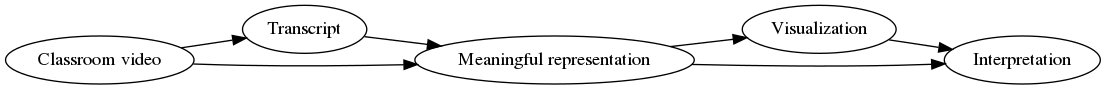
\includegraphics[width=\linewidth]{../figures/teacher_talk_manual_pipeline.png}
  \caption{Teacher talk analysis has a common manual pipeline. Classroom video is transcribed, meaningfully coded and then visualized and interpreted.}
  \label{fig:manualpipeline}
\end{figure}
%--------------------------------------------------------------------------------

A common theme in analysing teacher talk is that the pipeline illustrated in figure \ref{fig:manualpipeline} is manually done. This is obviously a laborious manual task that is prone to errors and is impractical in day-to-day teacher education. While analysing dialogic interactions in teacher talk require interpretation of what the teacher meant \parencite{viiriTeacherTalkPatterns2006}, analysing content structure in teacher talk was less subjective and was not as heavily based on interpretation of what the teacher meant \parencite{helaakoskiContentContentStructure2014}. This makes the content structure of teacher talk a prime candidate for automatic analysis of physics instruction quality using NLP methods. 


%--------------------------------------------------------------------------------


\chapter{Teacher talk as data}
\label{chap:speech}
\section{Audio data}
Automatic speech recognition (ASR), sometimes called speech to text, is a classification task, where the goal is to predict what was said from the audio signal of speech. Early ASR systems had an acoustic model which detected different sounds also known as phonemes to recognize numbers, some vowels and consonants for a single speaker \parencite{juangAutomaticSpeechRecognition2005}. Improvements in the acoustic model allowed for introduction of speaker-independent ASR \parencite{benzeghibaAutomaticSpeechRecognition2007,juangAutomaticSpeechRecognition2005}. The later addition of a language model based on statistical grammar and syntax helped more accurately predict the correct word based on what words previously appeared in the sentence \parencite{juangAutomaticSpeechRecognition2005}. Modern ASR systems utilize the fact that sentences are sequences of words and words are sequences of phonemes \parencite{bengioWordEmbeddingsSpeech2014}. 

Sequence based models such as Hidden Markov Models (HMM) are most commonly used, but deep learning approaches using Recurrent Neural Networks (RNN) and Long Short-Term Memory (LSTM) networks gaining popularity for acoustic models, language models and end to end text-to-speech models \parencite{bengioWordEmbeddingsSpeech2014,enarviAutomaticSpeechRecognition2017}. Deep learning approach is more data-driven and relies on fewer assumptions, but instead requires more data for training \parencite{bengioWordEmbeddingsSpeech2014}. This might be impractical if training data is limited. Depending on the architecture, an ASR system might be capable of either transcription, keyword spotting or both \parencite{juangAutomaticSpeechRecognition2005,enarviAutomaticSpeechRecognition2017}.

ASR is a difficult machine learning task because of a large search space, large vocabulary, undetermined length of word sequences and problems related to aligning speech signal to the text \parencite{enarviAutomaticSpeechRecognition2017}. Speech is highly variable even with a single speaker due to noise, but different pronunciations and accents mean that the audio signal will be different despite the same words being spoken \parencite{juangAutomaticSpeechRecognition2005}. Accents, dialects, emotional state, gender and casual speech slurring in spontaneous speech bring a lot of variation which makes conversational speech especially difficult compared to standard pronunciations and vocabulary \parencite{benzeghibaAutomaticSpeechRecognition2007, juangAutomaticSpeechRecognition2005}. Speaker-dependent systems are typically more accurate than speaker-independent systems \parencite{benzeghibaAutomaticSpeechRecognition2007,enarviAutomaticSpeechRecognition2017}.





\section{Text data}
TODO: NLP overview \parencite{silfverbergFinnPosOpensourceMorphological2016, kanervaTurkuNeuralParser2018}


\section{Finnish language}
TODO: Conversational vs official Finnish
Finnish language is particularly difficult for ASR because words are formed by concatenating smaller \parencite{enarviAutomaticSpeechRecognition2017}


%--------------------------------------------------------------------------------


\chapter{Methods}


\section{Dataset}

%--------------------------------------------------------------------------------
\begin{table}[]
  \begin{tabular}{ | l | l | l |}
  \hline
  \textbf{Start} & \textbf{End}  & \textbf{Text} \\ \hline
  10.0 & 15.0 & hehkulamppua kakstoista tunteesta kirjottaas taas että miten tuo laske\\ \hline
  15.0 & 20.0 & virtapiirejä virtapiirejä rakettien kans vaikka kuinka paljon tähän\\
  \hline
  \end{tabular}
  \caption{The sometimes inaccurate transcript consists of start and end times of the split and the utterance spoken by the teacher during that split.}
  \label{table:transcript}
\end{table}
%--------------------------------------------------------------------------------


The dataset consists of audio recordings of Finnish physics teachers in comprehensive schools collected during the Quality of Physics Instruction study \parencite{fischerQualityInstructionPhysics2014,helaakoskiContentContentStructure2014}. Helaakoski and Viiri \parencite*{helaakoskiContentContentStructure2014} used microphones attached to 25 physics teachers to record lessons on the topic of \enquote{Relation between electrical energy and power}. Of the 25 teachers, 22 taught their topic in two 45 min lessons and 3 teachers taught their topic during a 90 minute double lesson. 

In addition to audio recordings from the teachers, the students were tested on the knowledge of the topic before and after the lesson and a list of physics keywords was obtained from a physics book glossary. The audio data was then automatically transcribed using AaltoASR in 5 second splits \parencite{hirsimakiImportanceHighOrderNGram2009} as shown in table ~\ref{table:transcript}. We will define a transcript as a \emph{document} and the full collection of transcripts as \emph{corpus} of documents.



\section{Text Normalization}

%--------------------------------------------------------------------------------
\begin{table}[]
  \begin{tabular}{ | l | l | l | l | }
  \hline
  \textbf{Word} & \textbf{Snowball stem} & \textbf{Voikko lemma} & \textbf{Translation} \\ \hline
  virta & vir & Virta & current\\ \hline
  virtaa & virt & virrata & current\\ \hline
  virtapiiri & virtapiir & virtapiiri & electric circuit\\ \hline
  virtapiirejä & virtapiir & virtapiiri & electric circuits\\
  \hline
  \end{tabular}
  \caption{Both the Snowball stem and the Voikko lemma have problems with synonyms: the word "current" \emph{virtaa} is confused with the word "to flow" \emph{virrata} when lemma \emph{virta} was expected.}
  \label{table:stemmer}
\end{table}
%--------------------------------------------------------------------------------

First we apply text normalization techniques to the documents. First the documents are tokenized split by split into sequences of words using the NLTK tokenizer \parencite{birdNaturalLanguageProcessing2009}. Because of the agglutinative nature of Finnish, we then use the NLTK Snowball stemmer \parencite{birdNaturalLanguageProcessing2009} and the Voikko morphological analyser \parencite{pitkanenVoikkoFreeLinguistic2019}  for stemming and lemmatization. An example of the stems and lemmas obtained is shown in table ~\ref{table:stemmer}. We then process the physics keyword list in the same way. 


\section{Network analysis}

Expanding upon the idea of visualizing concept structure using conceptual networks by Helaakoski and Viiri \parencite*{helaakoskiContentContentStructure2014}, we automatically generate weighted networks using the physics keyword list. In addition to obtaining a visualization of the content structure of the teacher talk during the lesson, we compute network measures to quantify the relationships between the concepts.

We first compute a physics concept co-occurrence matrix for each text normalized lesson using an overlapping window over the splits produced by the ASR system. Since a non-overlapping window would not count two concepts occurring together but in different windows as co-occurring, we count the co-occurrences within the first half of the window and then add the co-occurrences between the two halves. This is done to avoid counting the same co-occurrence within a window twice due to the overlapping window.

We then represent a pair of co-occurring physics concepts as nodes with the amount of co-occurrences as the weight for that edge. Using NetworkX \parencite{hagbergExploringNetworkStructure2008} we can visualize the lessons concept structure as a network of concepts as shown in figure TODO.

\section{Time series analysis}

Temporal analysis of teacher talk is still problematic \parencite{lehesvuoriVisualizingCommunicationStructures2013}, which is why we also analyse the talk using time series analysis. For this we must first represent the teacher talk of the lesson as a time series, before computing a matrix profile for pattern recognition purposes.

This is done by computing a keyword frequency time series for each lesson using a fixed window over the splits generated by the ASR system. We count the total amount of keywords and amount in each category in each window. Physics keywords categorized as physics \emph{concepts} such as \emph{power}, physics related \emph{objects} such as \emph{battery}, physics \emph{units} such as \emph{watt}, \emph{meta} words such as \emph{theory} or \emph{other} words such as \emph{write}.


\chapter{Results and conclusions}


TODO:
\chapter{Related work}

Caballero et al. \parencite*{caballeroASRClassroomToday2017} applied ASR and NLP techniques to analyse teacher talk in Spanish and Finnish in a pilot study to determine the feasibility of the approach and maturity of modern ASR systems. Two teachers were equipped with microphones and concept networks were created and visualized by counting which physics concept keywords occurred together in the teacher's talk. We expanded upon this idea by using a larger dataset with more teachers, using alternative NLP methods such as lemmatization in addition to stemming, adding more representations of the data and including taking the temporal aspect of the lesson into account in the analysis and visualizations.

Fan et al. \parencite*{fanCourseMIRROREnhancingLarge2015} used NLP techniques to improve interactions between the student and the instructor. They developed a pilot system to collect self-reflections from the students, summarize them using NLP and then show the summaries to the instructors through a graphical interface. We believe that a simple to use interface to show summaries is necessary for teachers and developed visualizations so that teachers can see the content structure of the entire lesson at a glance.



\chapter{Discussion}

Research is being done in collaboration with the Department of Teacher Education at University of Jyväskylä and Centro de Investigación Avanzada en Educación (CIAE) at University of Chile.
 
\printbibliography

\end{document}
